\documentclass[11pt,a4paper]{article}

\usepackage[T1]{fontenc}
\usepackage[utf8]{inputenc}
\usepackage{lmodern}
\usepackage[margin=1in]{geometry}
\usepackage{parskip}
\usepackage{amsmath}
\usepackage{graphicx}
\usepackage{float}
\usepackage{booktabs}
\usepackage[table]{xcolor}
\usepackage[font=it,labelfont=it]{caption}
\usepackage{listings}
\usepackage{cite}
\usepackage[hidelinks]{hyperref}

\emergencystretch=2em

% highlighted best result in Table 1
\definecolor{bestbg}{RGB}{248,215,215}
\newcommand{\best}[1]{\cellcolor{bestbg}{\boldmath$#1$}}

% results that are still to be filled in
\newcommand{\pending}[1]{\textcolor{red}{[#1]}}
\newcommand{\pendingbox}{\fbox{\parbox[b][0.40\textwidth][c]{0.21\textwidth}{\centering\pending{pending}}}}

% code listings (Appendix B)
\definecolor{codegray}{gray}{0.45}
\definecolor{codegreen}{RGB}{0,110,40}
\definecolor{codeblue}{RGB}{0,60,160}
\definecolor{codered}{RGB}{160,40,40}
\lstset{
  language=Python,
  basicstyle=\ttfamily\scriptsize,
  keywordstyle=\color{codeblue},
  commentstyle=\color{codegreen},
  stringstyle=\color{codered},
  numbers=left,
  numberstyle=\tiny\color{codegray},
  numbersep=8pt,
  xleftmargin=2em,
  breaklines=true,
  breakatwhitespace=false,
  columns=fullflexible,
  keepspaces=true,
  showstringspaces=false,
  tabsize=4,
  frame=single,
  rulecolor=\color{codegray},
}

\title{How Effective Can Exposure Compensation Reduce Floating Artifacts in 3D Gaussian Splatting for Indoor Scene Reconstruction?}
\author{Kailun Li}
\date{}

\begin{document}

\maketitle
\thispagestyle{empty}

\tableofcontents
\clearpage

\section{Abstract}

Indoor scene reconstruction from casual imagery is hard to achieve because most of the images that are used as dataset are composed of shiny textures such as windows, wardrobes and plants, which results in complex lighting for the model to reconstruct. This problem is significant for real-world 3D reconstruction used in AR (Augmented Reality) applications, creation of metaverse, digital twin and gaming scene design, where photorealistic qualities of indoor scenes are required. In this paper, I study neural rendering methods (NeRF, Luminance-GS, 3DGS, etc.) and identify three improvement directions specifically for the 3DGS pipeline: (1) enhancing planar regions' depth accuracy with additional geometric constraints, (2) compensating for exposure differences across images, and (3) densifying the initial point cloud with multi-view data. This project then adapts the 3DGS technique to indoor environments by implementing exposure compensation into the reconstruction pipeline. By addressing exposure variation between input images, I try to reduce the floating artifacts (semi-transparent elliptical Gaussians) that often arise from lighting inconsistencies. The implementation gives every Gaussian a learnable exposure factor and renders these factors into an exposure map that normalizes brightness across training images, thereby making the optimisation less affected to lighting issues. \pending{Summary of the quantitative and qualitative results.} Therefore, I draw conclusions and identify the areas that can be improved.

\clearpage
\section{Introduction}

\subsection{What is Computer Vision and Development of NeRF and 3DGS}

Computer vision is a broad field enabling computers to interpret and recreate aspects of the visual world. One crucial branch is 3D scene reconstruction, where the goal is to recover a three-dimensional representation of a scene from images or video. Traditional approaches like photogrammetry use Structure-from-Motion (SfM) and Multi-View Stereo to produce point clouds and meshes from overlapping photos \cite{ref1}. In recent years, neural rendering techniques have revolutionised this area by learning implicit scene representations that can generate highly realistic novel views. This breakthrough work is Neural Radiance Fields (NeRF) \cite{ref2}, which represents a scene as a continuous volumetric function (density and color) encoded by a neural network. NeRF demonstrated that optimizing a coordinate-based MLP (multi-layer perceptrons) on a set of posed images can synthesize new views with high fidelity. This breakthrough drives rapid development of more efficient and robust variants. For example, Instant Neural Graphics Primitives (Instant-NGP) \cite{ref3} introduced a multi-resolution hash grid encoding that drastically accelerates training speed without quality loss, enabling high-fidelity NeRF models to be trained with much faster speed (hours to minutes) and rendered at an acceptable rates. Most recently, 3D Gaussian Splatting (3DGS) \cite{ref4} emerged as a new method blending explicit and implicit representations. Instead of a neural network, 3DGS represents the scene with millions of explicit 3D Gaussian primitives, which are optimized to fit the input images and can be rasterized in real time. This development of NeRF to Instant-NGP to 3DGS marks a progression toward faster and more direct reconstruction methods, thereby moving from heavy neural networks toward light-weight, explicit point-based models that preserve NeRF's quality while achieving real-time rendering.

\subsection{Modern Reconstruction Pipeline Overview}

Modern digital scene reconstruction pipelines combine image capture, computer vision processing, and graphics rendering to create usable 3D models from the real world. A typical pipeline begins with data acquisition, where a series of photographs or a video of the target scene is captured (often covering the environment from many angles). In professional setups for AR applications \cite{ref19}, additional sensors like depth cameras, LiDAR (laser scanning) \cite{ref5}\cite{ref20}, or SLAM (simultaneous localization and mapping) systems \cite{ref21} may be used to obtain wide range of composed initial spatial information. Next is a mapping and alignment stage: methods such as SfM (Structure from Motion) \cite{ref6} or SLAM estimate the camera poses for all images and generate a sparse point cloud of the scene. For instance, algorithms like COLMAP (which being used in 3DGS and NeRF) can automatically detect feature points across images, match them, and solve for 3D point positions and camera parameters. The sparse reconstruction may be enhanced by densification (multi-view stereo) or by merging depth sensor data, creating a more complete point cloud or mesh of the scene. With the inputs aligned in 3D, the pipeline then feeds into a reconstruction algorithm such as NeRF or 3DGS. In a NeRF-based pipeline, the posed images train a neural radiance field, which can later render in a camera direction that isn't in the original input images via volumetric ray marching. In a 3DGS pipeline, the initial point cloud seeds a set of Gaussian primitives that are optimized/ trained by comparing rendered and real images. This core optimisation stage produces a digital twin of the scene, a model that can be stored or processed. The final step is deployment of the reconstructed scene in the desired platform. For example, the optimized Gaussians or a mesh extracted from them can be imported into a 3D engine.

\subsection{What is 3DGS, why it is valuable for its role in the Pipeline}

\begin{figure}[H]
\centering
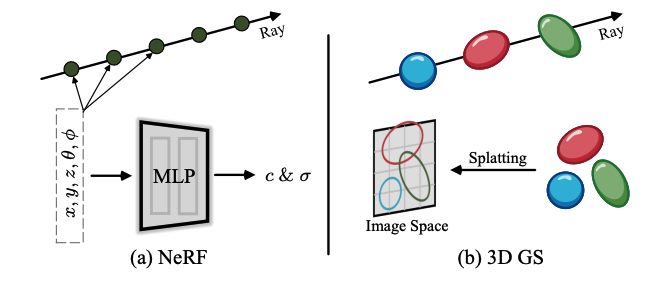
\includegraphics[width=0.72\textwidth]{figures/fig1_nerf_vs_3dgs.png}
\caption{NeRFs vs. 3D GS. (a) NeRF samples along the ray and then queries the MLP to obtain corresponding colors and densities, which can be seen as a backward mapping (ray tracing). (b) In contrast, 3D GS projects all 3D Gaussians into the image space (i.e., splatting) and then performs parallel rendering, which can be viewed as a forward mapping (rasterization). Image and comment taken from \cite{ref9}}
\label{fig:1}
\end{figure}

In the pipeline described above, 3DGS proposed a new way of reconstructing 3D models without using neural network (MLP) in NeRF. The major difference is 3D Gaussian Splatting models the scene as a large collection of elliptical 3D Gaussian blobs in 3D space. Each Gaussian is defined by parameters specifying its center location, its spatial covariance (which can be thought of as the extent and orientation of the blob) and its appearance (color and opacity) \cite{ref7}. Because these Gaussians are explicit primitives (much like tiny 3D ``splats'' or particles), the scene can be rendered by rasterizing them -- projecting each Gaussian onto the image plane and blending their contributions \cite{ref8}, rather than tracing rays through a neural field. Details of the mathematical basis of 3DGS are given in Appendix A. This offers a significant speed advantage: the original 3DGS work achieved real-time ($>$30 FPS) 1080p rendering, something standard NeRF cannot do due to its neural network learning process. Another advantage of 3DGS is quality: by optimizing millions of parameters (that forms the Gaussians) directly with image-based losses, it can produce sharp, photorealistic results comparable to or better than NeRF\cite{ref4}. Within a reconstruction pipeline, 3DGS thus enables faster scene digitization: one can capture a space, run the 3DGS optimization, and almost immediately have a model ready to visualize or integrate into applications. This makes it highly appealing for time-sensitive applications where both speed and fidelity are required. Finally, because 3DGS contains an interpretable collection of primitives, it is easy to further edit or refine the model with 3D editors (e.g. deleting a few Gaussians to clean up artifacts), which is harder to do with opaque neural network weights.

\section{Limitations of Original 3DGS and Researching Directions}

\begin{figure}[H]
\centering
\begin{tabular}{@{}cccc@{}}
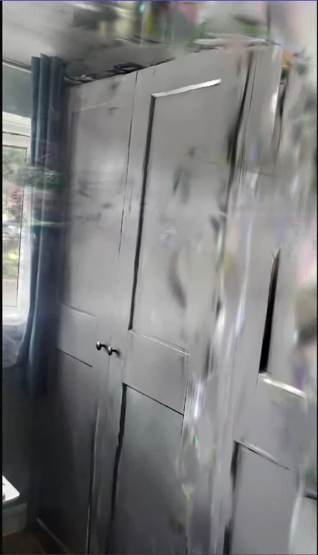
\includegraphics[width=0.235\textwidth]{figures/fig2_1_3dgs2023.png} &
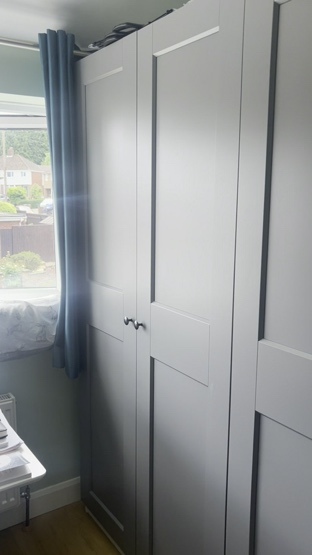
\includegraphics[width=0.235\textwidth]{figures/fig2_2_groundtruth.jpg} &
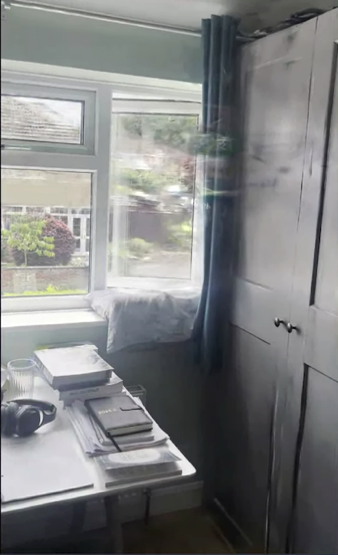
\includegraphics[width=0.235\textwidth]{figures/fig2_3_3dgs2023.png} &
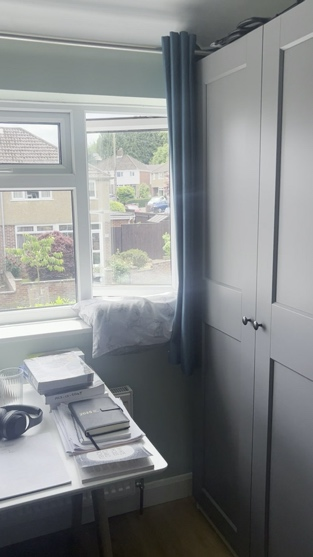
\includegraphics[width=0.235\textwidth]{figures/fig2_4_groundtruth.jpg} \\
3DGS 2023 & Ground Truth & 3DGS 2023 & Ground Truth
\end{tabular}
\caption{A direct comparison between original 3DGS model output running in SIBR viewer (A model render viewer for 3DGS) (left) with the ground truth image that is used as dataset (right) where the problem of inaccurate plane geometry and floating artifacts are shown while reconstructing wardrobe (planar regions)}
\label{fig:2}
\end{figure}

Here I have created a dataset by using iPhone camera to video my room in 360 degrees and then process the video by cropping into images by frames, then feed those images into COLMAP algorithm to extract camera positions and parameters for 3DGS to train. By observing the outcome model, I then look into the causes that produce those `ripped' reconstruction quality and figuring out what are the current researching directions to improve the quality.

(1) Local Optimal: Due to the unstructured and irregular nature of Gaussian point clouds, it is difficult to ensure geometric reconstruction accuracy and multi-view consistency by relying solely on image reconstruction loss. Optimization based solely on image reconstruction loss can easily lead to local optimality, which ultimately causes the Gaussian to not conform to the actual surface and exhibit poor geometric accuracy (Figure~\ref{fig:2}). In novel views, one might observe ``floating'' blobs above a flat surface due to this ambiguity. Therefore, there should be more parameters to be introduced. Recent works address this by adding geometric constraints. For example, Deng et al. introduced DS-NeRF \cite{ref10}, which uses known 3D points from SfM to supervise the NeRF's density learning -- a concept that could likewise guide 3DGS to correct its geometry. Chen et al. propose a planar 3DGS (PGSR) \cite{ref11,ref28} that explicitly leverages room layout: they initialize Gaussians on detected large planes and enforce those to stay flat, which significantly reduces floaters and generates more accurate walls. Such plane regularization and depth supervision techniques help to ensure the reconstructed model aligns better with real geometry.

(2) Lighting Inconsistencies and Exposure Artifacts: Standard 3DGS assumes the input images are radiometrically consistent (same exposure, lighting conditions). In real indoor captures, auto-exposure and varying lighting can cause the same surface to appear with different brightness in different images. The optimization, lacking an exposure model, may explain these differences by introducing semi-transparent densities (floating artifacts) that account for brightness changes (Figure~\ref{fig:2}). This problem was appeared in NeRF as well and became one of the major researching directions. NeRF in the Wild (NeRF-W) \cite{ref12,ref22,ref23,ref24} pioneered the idea of per-image appearance variables to model exposure and lighting variations. In the context of 3DGS, recent research integrates exposure compensation models to normalize or learn the exposure differences. For instance, luminance-GS \cite{ref13} quickly rewrites every camera photo so they all look like they were shot with the same, normalised exposure. So, no ultra-light and dark places exist because of different lightnings. With those balanced photos, 3-D Gaussian Splatting can learn shapes and colours without getting confused by dark or blown-out views. When you render new angles, it shows the corrected colours, so images stay evenly lit and don't flicker.

(3) Sparse Initialization in Low-Texture Areas: Because 3DGS builds on a sparse SfM point cloud, its performance is tied to the quality of that initial reconstruction. In scenes with low-texture or repetitive patterns (e.g. blank walls, white ceilings, or even areas with moving foliage like some indoor plants), SfM often fails to produce enough points. The resulting Gaussian representation may have ``holes'' or rely on the optimization to fill in large gaps with little guidance (Figure~\ref{fig:2}). This can manifest as unstable geometry or poor coverage of certain surfaces. To address this, researchers explore methods to improve the initial point density. 360-GS \cite{ref14,ref25,ref26,ref27} integrates multi-view stereo depth maps or neural depth predictors to add more points in texture-less regions before starting 3DGS optimization. Another approach is to relax the dependence on SfM entirely: for example, a recent SfM-free 3DGS \cite{ref15} method jointly estimates camera poses and Gaussians via hierarchical training on video input. On top of that, the creation of SfM point cloud can be improved by using a radar laser scanner for the creation of dataset, so it can pick up all the geometric shape of the scene. Hence guiding the SfM generations \cite{ref20}.

\section{A Novel Exposure Compensation}

\subsection{Overview of adaptation pipeline}
\label{sec:overview}

\begin{figure}[H]
\centering
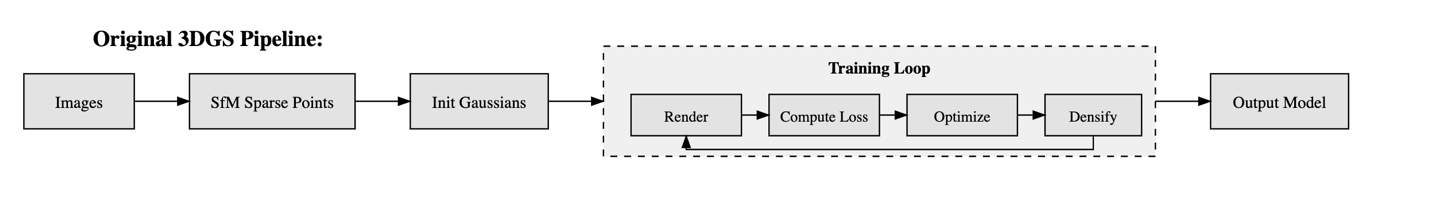
\includegraphics[width=\textwidth]{figures/fig3_original_pipeline.png}\\[1ex]
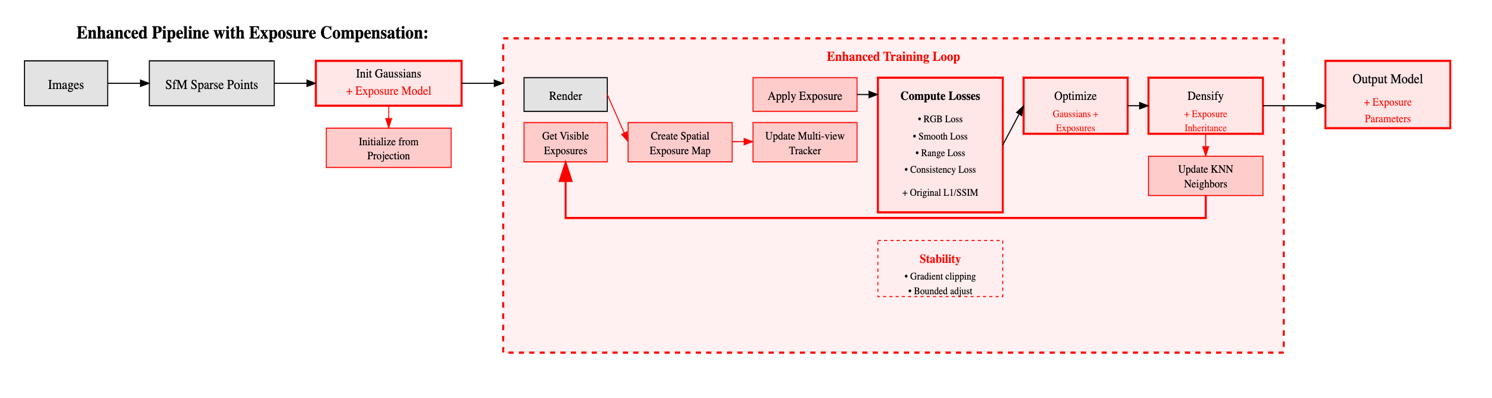
\includegraphics[width=\textwidth]{figures/fig3_enhanced_pipeline.png}
\caption{An overview of the designed pipeline}
\label{fig:3}
\end{figure}

Based on the three directions evaluated in the previous section, I am implementing a novel exposure compensation method for the 3DGS pipeline. Rather than normalising exposure by rewriting input images using a colour matrix as in Luminance-GS, I introduce a new exposure parameter that is stored on every Gaussian. Since exposure during capture can cause smooth surfaces to appear very bright from some angles (due to light reflection) and dark from others, adding exposure factors lets the model keep how much light falls on a surface separate from the colour of the surface itself. During the learning optimisation phase, these exposure parameters are rendered into an exposure map that relates the colours predicted by the Gaussians to the ground-truth values before computing gradient losses, reducing the influence of lighting variations.

Here I add exposure factors and their components to the original 3DGS pipeline, replacing its assumption of global photometric consistency across all training views. In my implementation, every Gaussian receives an exposure factor during the initialisation stage, stored in the tensor (the PyTorch-style matrix that holds a Gaussian's properties) alongside its position, colour and opacity. I set this factor by sampling the grey-scale intensity of each Gaussian's image projections---analogous to how 3DGS bootstraps colour from mean observations, but exposure-specific, because grey (between black and white) reflects how much light falls on the Gaussian. Because the colour that SfM gives to a point already contains this brightness, I divide the starting colour of each Gaussian by its exposure factor, so that colour multiplied by exposure still reproduces what the camera saw.

After rendering, I use the exposure factors of all visible Gaussians to construct a spatial exposure map. Instead of approximating this map, I render it: the rasteriser of 3DGS can splat any per-Gaussian value in place of the colour, so a second pass in which the colour of every Gaussian is replaced by its exposure factor accumulates the exposure values with exactly the same alpha-compositing weights as the colour image. Dividing by the accumulated weight then gives, for every pixel, the average exposure of the Gaussians that cover it. The result is a pixel-accurate exposure map that reflects how each 3D primitive influences each pixel. This map links the exposure-affected values of the ground-truth images to the exposure-free values that the Gaussians learn (see section~\ref{sec:render}). That adjustment is the core of my adaptation: it removes the non-uniform colour/brightness caused by camera position from the target colours the Gaussians must learn. During this second pass the position, shape and opacity of the Gaussians are held fixed, so that the exposure map can only be explained by the exposure factors and not by moving the geometry.

To ensure multi-view consistency, I keep a tracker that stores, for each Gaussian, the exposure factor it had in the most recent views in which it was visible; a later consistency loss encourages these factors to converge. Spatial coherence uses the K-nearest-neighbour (KNN) structure \cite{ref29} I introduce later, which assumes nearby 3-D points share similar lighting. A smooth\_loss term penalises exposure differences between the neighbours found by KNN.

During training I compute several losses involving the exposure factors, yielding more accurate gradients (see section~\ref{sec:losses}) for optimisation. Because the exposure factor is a property of the Gaussian itself, it follows the Gaussian through densification: after every densification step, newly created Gaussians inherit their parent's exposure factor exactly and are then optimised on their own, and the factors of pruned Gaussians are removed together with them.

Although each exposure factor is only one float per Gaussian, the losses that involve them have to be evaluated at every iteration ($\sim$30\,000 iterations for a good model). My first attempt looped over the Gaussians in Python to compute the neighbour and multi-view terms, which is memory-intensive and significantly lengthens training time.

\begin{figure}[H]
\centering
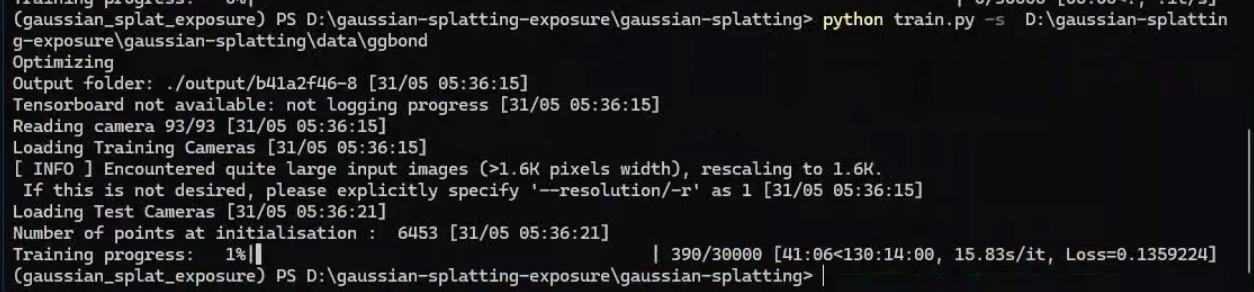
\includegraphics[width=\textwidth]{figures/fig4_slow_iterations.png}
\caption{During the 390 iterations, it is already taking 15.83s per iteration. For 30000 iterations it will take hundreds of hours to train.}
\label{fig:4}
\end{figure}

\begin{figure}[H]
\centering
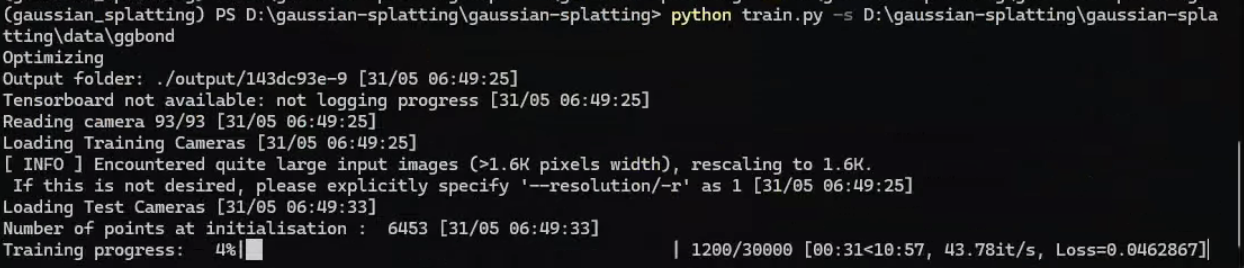
\includegraphics[width=\textwidth]{figures/fig5_normal_speed.png}
\caption{Normal speed for early iterations (43.78 iterations per second)}
\label{fig:5}
\end{figure}

Therefore, I wrote every exposure computation as tensor operations that run on the GPU together with the rest of the pipeline. The exposure map is produced by the rasteriser itself, the smoothness loss is evaluated on a random sample of the visible Gaussians at each iteration, and the multi-view tracker is a buffer of fixed size. By doing this, the cost of the exposure terms no longer depends on a Python loop over every Gaussian, so the training time is shortened and less compute is required.

\subsection{Implementation for Exposure modules}

\subsubsection{Exposure\_gaussians.py -- Core Exposure Model}

This file (see Appendix B) implements the fundamental exposure model that manages per-Gaussian exposure factors ($e_i$). The \textit{ExposureGaussianModel} class extends the Gaussian model of 3DGS with one learnable exposure parameter for each Gaussian, clamped between 0.05 and 1.5 to maintain stability, and registers it in the same Adam optimiser (a stochastic-gradient algorithm widely used in machine learning) \cite{ref16} as the other properties of the Gaussian.

The key functions include:

\begin{itemize}
\item \texttt{initialise\_exposure()}: Sets the starting exposure values and divides the starting colours by them
\item \texttt{densify\_and\_clone()}, \texttt{densify\_and\_split()} and \texttt{densification\_postfix()}: Record which Gaussians are being cloned or split, so that each new Gaussian copies the exposure factor of its parent
\item \texttt{prune\_points()}: Removes the exposure factors, tracker entries and neighbour lists of pruned Gaussians
\item \texttt{update\_exposure\_history()}: Stores the current exposure of the visible Gaussians in the multi-view tracker
\item \texttt{rebuild\_neighbors()}: Recomputes the KNN neighbour list of every Gaussian
\end{itemize}

\subsubsection{Exposure\_factors.py}

This file computes the initial exposure values from the training images:

\begin{itemize}
\item \texttt{rgb\_to\_gray()}: Converts RGB images to grayscale using standard luminance weights
\item \texttt{sample\_gray\_from\_images()}: Projects the Gaussians into every training image and samples grayscale values at the projected positions using grid sampling.
\item \texttt{initialize\_exposure\_from\_projection()}: Initializes exposure values by averaging the grayscale intensities over all the images in which a Gaussian appears. Gaussians that appear in no image receive a default value of 0.95
\end{itemize}

\subsubsection{Exposure\_render.py and Exposure\_adjustment.py}
\label{sec:render}

These modules create the exposure map and handle the actual adjustment of colors using exposure factors:

\begin{itemize}
\item \texttt{render\_exposure\_map()}: Renders the exposure factors into the spatial exposure map by passing them to the rasteriser in place of the colour and dividing by the accumulated opacity, which gives the average exposure of the Gaussians covering each pixel. Pixels that no Gaussian covers receive a neutral exposure of 1
\item \texttt{adjust\_color\_with\_exposure()}: The function that expresses exposure normalization using the formula:
\begin{equation}
\label{eq:1}
C_{\mathrm{adj}} = \frac{C}{e + \varepsilon}
\end{equation}
where:

\begin{tabular}{@{}r@{${}={}$}l@{}}
$C_{\mathrm{adj}}$ & Exposure-free Colour Map for Ground Truth \\
$C$ & Exposure-dependent Colour Map for Ground Truth \\
$e$ & Exposure Map \\
$\varepsilon$ & 0.0001 (help to prevent fraction grows to infinity)
\end{tabular}

\item \texttt{apply\_exposure()}: Applies the same relationship in the other direction, $C = C_{\mathrm{adj}} \cdot e$. During training I multiply the exposure-free rendered image by the exposure map and compare the result with the unmodified ground truth. This is equivalent to Equation~\ref{eq:1}, but if the ground truth were divided by the map instead, the loss could be reduced simply by increasing the exposure, since both sides of the comparison become darker
\item \texttt{render\_with\_exposure()}: Returns the exposure-free image, the exposure map and their product for one camera
\item \texttt{adjust\_depth\_with\_exposure()}: Modulates depth values based on exposure factors with either sigmoid or linear weighting (different formula for modulation)
\end{itemize}

\subsubsection{Exposure\_losses.py}
\label{sec:losses}

This file defines four specialized loss functions for exposure optimization:

\begin{itemize}
\item \texttt{exposure\_rgb\_loss()}: Computes MSE loss (pixel-wise mean-squared-error between the colour of a rendered view and the ground-truth photograph it should match) between exposure-adjusted rendered images and ground truth
\item \texttt{exposure\_smooth\_loss()}: Enforces spatial smoothness between neighboring Gaussians' exposure values, evaluated on a random sample of the visible Gaussians and their KNN neighbours
\item \texttt{exposure\_range\_loss()}: Regularizes exposure values to stay within [0.1, 1.0]
\item \texttt{exposure\_consistency\_loss()}: Ensures multi-view consistency by minimizing the variance of the exposure values that the same Gaussian had across the recent views stored in the tracker
\end{itemize}

\subsubsection{Neighbors.py}

This file computes the neighbour list used by the smoothness loss. It uses FAISS (a library that uses quantisation and inverted-file indices to perform fast, approximate nearest-neighbour searches) \cite{ref18} when a GPU version is available, and otherwise a KDTree (which recursively partitions 3D point space along axis-aligned planes to enable exact nearest-neighbour queries) \cite{ref17}.

\subsubsection{Exposure\_\_init\_\_call.py}

This provides a unified interface that combines all exposure losses with configurable weights.

\subsection{Implementation in trainv1.py}

The 3DGS repository has a train.py file used to kick off training \cite{ref30}. The initial integration in trainv1.py (see Appendix B) introduces basic exposure compensation, where I added exposure support while postponing advanced features for clarity. At this stage the exposure factors are held in a small stand-alone \textit{ExposureModel} (also listed in Appendix B) rather than in the Gaussians themselves. After the Gaussian point cloud is loaded from SfM, ExposureModel(num\_gaussians) is instantiated (lines 33--36), and its parameters are given to an Adam optimiser. After rendering, the system creates an exposure map (initially simplified as a uniform map based on the mean exposure), applies the adjustment to the rendered image (lines 102--114), and includes the exposure loss in the total optimisation objective. There is also a simple exposure inherence implemented after densification, where the exposure tensor is resized by hand (lines 161--175). However, there is no actual neighbour computation (spatial smoothness disabled) in trainv1.py, as I only implemented an empty list for neighbour. Additionally, there is no multi-view consistency tracking, since I set the smooth and consistency losses to 0.

Nonetheless, I still ran this basic adaptation and noticed a noticeable improvement both quantitatively and qualitatively (see Table~\ref{tab:1}).

\subsection{Fully implementation in trainv2.py}

In trainv2.py, I implemented the complete version of the pipeline outlined in section~\ref{sec:overview}. The exposure factors are moved from the stand-alone \textit{ExposureModel} into the Gaussians (\textit{ExposureGaussianModel}), which replaces the manual resizing in trainv1.py. When 3DGS clones, splits or prunes Gaussians, the exposure factors are cloned, split and pruned with them, so each factor always belongs to the right Gaussian and new Gaussians start from their parent's value. Before training starts, the exposure values are initialised from the projected grey-scale intensities.

I also implemented a complete version of multi-view consistency tracking, which replaces the \textit{multiview\_exposure\_dict = \{\}} in trainv1.py. The tracker is a buffer that holds the last ten exposure values of every Gaussian and is updated each time the Gaussian is visible. Now my adaptation can track how each Gaussian's exposure behaves as different camera viewpoints update it over time, and this can be penalised by a consistency loss. I have also implemented an actual neighbour-computation system using KDTree \cite{ref17} and FAISS \cite{ref18}. The neighbour list is recomputed every 1000 iterations; in between, newly created Gaussians temporarily use their parent's neighbours.

For the exposure map, I changed from a uniform exposure map to the rendered spatial exposure map described in section~\ref{sec:overview}. Each training iteration therefore renders twice: once for the exposure-free colour image and once for the exposure map. The two are multiplied and compared with the ground truth using the original L1 and SSIM losses of 3DGS, to which the four exposure losses are added.

To keep the optimisation stable, only the RGB exposure loss is active during the first 1000 iterations, and the weight of the exposure losses increases linearly over the first 5000 iterations. The learning rate of the exposure factors starts at one tenth of its final value (0.001) for the first 3000 iterations and is then reduced by 2\% every 2000 iterations, and the gradient of the exposure factors is clipped. As mentioned earlier, due to slow training speed (Figure~\ref{fig:4}), the smoothness loss is computed on at most 50\,000 randomly chosen visible Gaussians per iteration, instead of inspecting every Gaussian each iteration; this makes it more memory-efficient. The densification of 3DGS is otherwise left unchanged, including its periodic opacity reset. I also added a variable that multiplies the gradient threshold of densification to control how many Gaussians can be added during each densification, together with switches that turn each exposure component off, so that the contribution of each part can be measured separately.

\subsection{Outcome and Achievement}

The most immediate benefit of modeling exposure as a per-Gaussian property is that illumination and surface appearance are stored separately. Without it, a Gaussian has to average between the different exposure levels of the same surface, resulting in muddy, inconsistent colors, or the optimisation introduces semi-transparent Gaussians to account for the brightness changes. By allowing each Gaussian to carry its own exposure factor, the system is able to disentangle illumination variations from true surface appearance: for objects that span both bright and shadowed regions, lighting differences can be absorbed by the exposure factors within the exposure map rather than being averaged into the surface color.

Building on this, the consistency loss deals with multi-view behaviour. Without it, the exposure factor of a single Gaussian seen under varying exposures across different training views is pulled toward a different value by each view's lighting. The consistency loss counteracts that by pushing every Gaussian toward a single, view-independent exposure, so that each Gaussian keeps a stable value regardless of which training view updated it last.

At the same time, spatial smoothness regularization encourages plausible exposure fields that respect the underlying geometry. Rather than each Gaussian choosing an unrelated exposure value, the smoothness loss encourages neighboring Gaussians to share similar exposure factors, which results in contiguous regions that correspond to real-world lighting phenomena. Because the exposure map is rendered directly from these factors, it can be saved and inspected for every view, which makes the reconstructed exposure more interpretable.

Training stability also benefits from the bounded factors. Every exposure factor is clamped between 0.05 and 1.5 and the range loss keeps the values inside [0.1, 1.0], so the exposure map can neither approach zero nor grow without limit. Because the map multiplies the rendered image instead of dividing the ground truth, no division by small values takes place during backpropagation, which is where exploding gradients would otherwise come from. Together with the gradient clipping and the warm-up of the exposure losses, this keeps the updates of the exposure factors bounded throughout training.

Memory efficiency is also considered in the multi-view tracker. Instead of storing full exposure histories for every Gaussian (which quickly becomes infeasible for large scenes or long training runs), the system retains only the ten most recent observations in a single tensor. In the same way, the smoothness loss only looks at a sample of the currently visible Gaussians, reducing both memory usage and computational overhead.

\subsection{Potential Improvement}

However, the current implementation in trainv2.py, while functional, still has limitations. The exposure map is obtained with a second rendering pass, which adds a second rasterisation to every iteration. A better improvement would involve modifying the CUDA rendering kernel to accumulate exposure values during the alpha compositing process of the colour pass itself. Currently, the renderer accumulates only color and opacity, but by extending it to track exposure contributions from each Gaussian at the same time, we could generate the same pixel-accurate exposure maps in a single pass. Beyond kernel modifications, the per-Gaussian scalar exposure model itself has limitations. Real-world illumination exhibits diverse structure: regional lighting variations, and local surface interactions, but a single value per Gaussian is the same in every image, so it cannot represent the camera changing its exposure from one image to the next. The initialisation also does not test whether a Gaussian is hidden behind another surface in an image, so its starting grey value can include views in which it is occluded.

The smoothness loss treats all neighbours equally. At an extreme exposure transition such as a window, where indoor and outdoor regions meet, neighbouring Gaussians can have very different exposure levels, and enforcing similar values across this boundary may create an intermediate zone that appears blurry. Reducing the smooth loss in such high-gradient regions, or identifying window regions and handling them specifically, would address this.

The current densification strategy also operates blindly to exposure variations, under-sampling regions with complex lighting transitions. An exposure-aware densification mechanism would monitor both geometric and photometric gradients, automatically increasing Gaussian density at shadow boundaries, specular highlights, and other areas where lighting changes rapidly. This adaptive sampling can therefore naturally allocate computational resources where they contribute most to visual quality.

\section{Results and Evaluation}

\begin{table}[H]
\centering
\caption{Quantitative evaluation of our method compared to original 3DGS code and their updated code in 2024 (introduce simple exposure compensation), computed over one dataset that has been created by me. SSIM (Structural Similarity Index Measure): Ranges from 0 to 1, where 1 indicates perfect structural similarity between images. PSNR (Peak Signal-to-Noise Ratio): Measured in decibels (dB), where higher values indicate better image quality.$\uparrow$ indicates that higher values are better for both metrics. All methods were evaluated at 30,000 iterations on the Room dataset with 56 test images. (More detailed result see appendix C)}
\label{tab:1}
\vspace{0.5ex}
\begin{tabular}{@{}lcccc@{}}
\toprule
Dataset & \multicolumn{4}{c}{Room} \\
\cmidrule(l){2-5}
Method\textbackslash Metric & \textit{SSIM}$\uparrow$ & \textit{SSIM Range} & \textit{PSNR}$\uparrow$ & \textit{PSNR Range} \\
\midrule
v1-30K & $0.9669 \pm 0.0168$ & $[0.9061, 0.9881]$ & $30.99 \pm 3.89$ & $[19.32, 36.66]$ \\
v2-30K & \pending{pending} & \pending{pending} & \pending{pending} & \pending{pending} \\
3DGS2023-30K & $0.9605 \pm 0.0208$ & $[0.9113, 0.9967]$ & $36.89 \pm 4.75$ & $[21.26, 44.50]$ \\
3DGS2024-30K & $0.9787 \pm 0.0173$ & $[0.9302, 0.9983]$ & $37.71 \pm 3.37$ & $[30.65, 45.07]$ \\
\bottomrule
\end{tabular}
\end{table}

\begin{figure}[H]
\centering
\begin{tabular}{@{}cccc@{}}
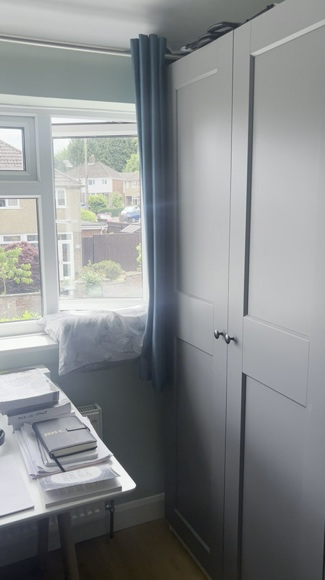
\includegraphics[width=0.235\textwidth]{figures/fig6_window_groundtruth.png} &
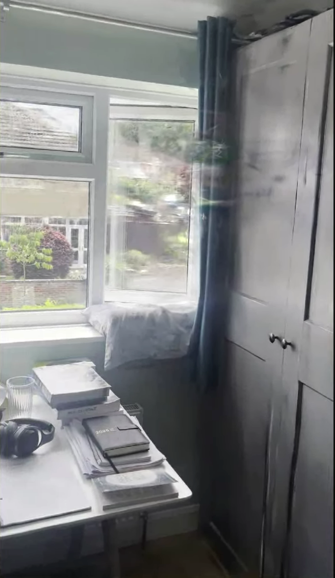
\includegraphics[width=0.235\textwidth]{figures/fig6_window_3dgs2023.png} &
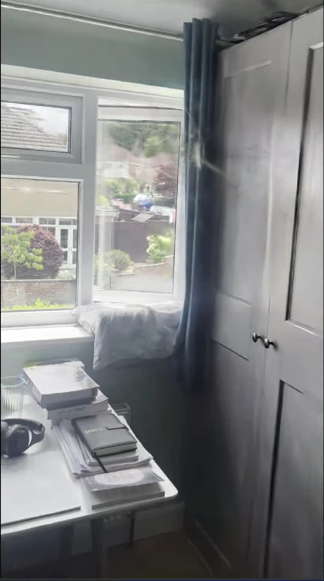
\includegraphics[width=0.235\textwidth]{figures/fig6_window_3dgs2024.png} &
\pendingbox \\
Ground Truth & 3DGS 2023 & 3DGS 2024 & Ours (v2) \\[1ex]
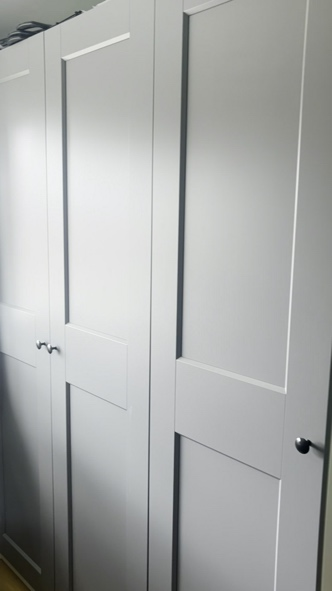
\includegraphics[width=0.235\textwidth]{figures/fig6_wardrobe_groundtruth.jpg} &
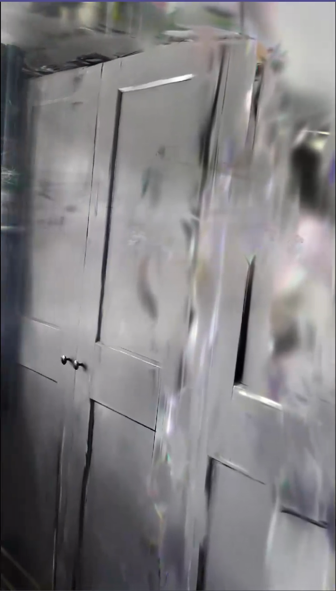
\includegraphics[width=0.235\textwidth]{figures/fig6_wardrobe_3dgs2023.png} &
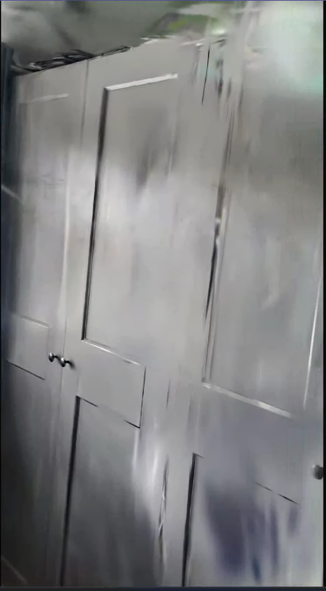
\includegraphics[width=0.235\textwidth]{figures/fig6_wardrobe_3dgs2024.png} &
\pendingbox \\
Ground Truth & 3DGS 2023 & 3DGS 2024 & Ours (v2)
\end{tabular}
\caption{Qualitative Comparisons of ground truth, 3DGS 2023, 3DGS 2024 and ours (v2) of two different scenes, Window/Wardrobe, under the same dataset Room}
\label{fig:6}
\end{figure}

All methods are trained for 30,000 iterations on the same dataset. For trainv2.py, the test images are rendered with the exposure map applied (render\_exposure.py in Appendix B), i.e. the exposure-free image multiplied by its exposure map, since this is the image that is compared with the ground truth during training.

\pending{Discussion of the quantitative and qualitative results of trainv2.py.}

\section{Conclusion}

This paper looked at the limitations of 3D Gaussian Splatting (3DGS) for indoor scene reconstruction and proposed an exposure compensation approach to address one of its key challenges. Through my analysis and novel implementation for exposure compensation, I have integrated exposure normalization into the 3DGS pipeline: every Gaussian carries a learnable exposure factor that is initialised from the training images, inherited through densification, rendered into a pixel-accurate exposure map and regularised by smoothness, range and multi-view consistency losses. \pending{Summary of the findings of Section 5.} In the end, I have also addressed the possible ways of improvement for the exposure compensation method.

\clearpage
\phantomsection
\addcontentsline{toc}{section}{References}
\begin{thebibliography}{30}

\bibitem{ref1}
Fang, K., Zhang, Q., Wan, C. et al. Single view generalizable 3D reconstruction based on 3D Gaussian splatting. Sci Rep 15, 18468 (2025). \url{https://doi.org/10.1038/s41598-025-03200-7}

\bibitem{ref2}
Mildenhall B, Srinivasan PP, Tancik M, Barron JT, Ramamoorthi R, Ng R. Nerf: Representing scenes as neural radiance fields for view synthesis. Communications of the ACM. 2021 Dec 17;65(1):99-106.

\bibitem{ref3}
Müller T, Evans A, Schied C, Keller A. Instant neural graphics primitives with a multiresolution hash encoding. ACM transactions on graphics (TOG). 2022 Jul 22;41(4):1-5.

\bibitem{ref4}
Kerbl B, Kopanas G, Leimkühler T, Drettakis G. 3d gaussian splatting for real-time radiance field rendering. ACM Trans. Graph.. 2023 Aug 1;42(4):139-.

\bibitem{ref5}
Li Y, Ibanez-Guzman J. Lidar for autonomous driving: The principles, challenges, and trends for automotive lidar and perception systems. IEEE Signal Processing Magazine. 2020 Jun 29;37(4):50-61.

\bibitem{ref6}
J. L. Schönberger and J. -M. Frahm, ``Structure-from-Motion Revisited,''~2016 IEEE Conference on Computer Vision and Pattern Recognition (CVPR), Las Vegas, NV, USA, 2016, pp. 4104-4113, doi: 10.1109/CVPR.2016.445.

\bibitem{ref7}
Plainconcepts 3D Gaussian Splatting Review \url{https://plainconcepts.com/3d-gaussian-splatting/#:~:text=parameters%3A}

\bibitem{ref8}
M. Zwicker, H. Pfister, J. van Baar and M. Gross, ``EWA volume splatting,'' Proceedings Visualization, 2001. VIS '01., San Diego, CA, USA, 2001, pp. 29-538, doi: 10.1109/VISUAL.2001.964490.

\bibitem{ref9}
Chen G, Wang W. A survey on 3d gaussian splatting. arXiv preprint arXiv:2401.03890. 2024 Jan 8.

\bibitem{ref10}
Deng K, Liu A, Zhu JY, Ramanan D. Depth-supervised nerf: Fewer views and faster training for free. InProceedings of the IEEE/CVF conference on computer vision and pattern recognition 2022 (pp. 12882-12891).

\bibitem{ref11}
D. Chen~et al., ``PGSR: Planar-based Gaussian Splatting for Efficient and High-Fidelity Surface Reconstruction,'' in~IEEE Transactions on Visualization and Computer Graphics, doi: 10.1109/TVCG.2024.3494046.

\bibitem{ref12}
Martin-Brualla R, Radwan N, Sajjadi MS, Barron JT, Dosovitskiy A, Duckworth D. Nerf in the wild: Neural radiance fields for unconstrained photo collections. InProceedings of the IEEE/CVF conference on computer vision and pattern recognition 2021 (pp. 7210-7219).

\bibitem{ref13}
Cui Z, Chu X, Harada T. Luminance-GS: Adapting 3D Gaussian Splatting to Challenging Lighting Conditions with View-Adaptive Curve Adjustment. arXiv preprint arXiv:2504.01503. 2025 Apr 2.

\bibitem{ref14}
Bai J, Huang L, Guo J, Gong W, Li Y, Guo Y. 360-GS: Layout-guided panoramic Gaussian splatting for indoor roaming. arXiv preprint arXiv:2402.00763. 2024 Feb 1.

\bibitem{ref15}
Ji B, Yao A. SfM-Free 3D Gaussian Splatting via Hierarchical Training. arXiv preprint arXiv:2412.01553. 2024 Dec 2.

\bibitem{ref16}
Kingma DP, Ba J. Adam: A method for stochastic optimization. arXiv preprint arXiv:1412.6980. 2014 Dec 22.

\bibitem{ref17}
J. H. Friedman, J. L. Bentley, and R. A. Finkel, ``An algorithm for finding best matches in logarithmic expected time,'' ACM Transactions on Mathematical Software (TOMS), vol. 3, no. 3, pp. 209--226, 1977.

\bibitem{ref18}
J. Johnson, M. Douze, and H. Jégou, ``Billion-scale similarity search with GPUs,'' IEEE Transactions on Big Data, vol. 7, no. 3, pp. 535--547, 2021.

\bibitem{ref19}
Venkatesan M, Mohan H, Ryan JR, Schürch CM, Nolan GP, Frakes DH, Coskun AF. Virtual and augmented reality for biomedical applications. Cell Rep Med. 2021 Jul 21;2(7):100348. doi: 10.1016/j.xcrm.2021.100348. PMID: 34337564; PMCID: PMC8324499.

\bibitem{ref20}
Zheng C, Xu W, Zou Z, Hua T, Yuan C, He D, Zhou B, Liu Z, Lin J, Zhu F, Ren Y. Fast-livo2: Fast, direct lidar-inertial-visual odometry. IEEE Transactions on Robotics. 2024 Nov 19.

\bibitem{ref21}
Huang H, Li L, Cheng H, Yeung SK. Photo-slam: Real-time simultaneous localization and photorealistic mapping for monocular stereo and rgb-d cameras. InProceedings of the IEEE/CVF Conference on Computer Vision and Pattern Recognition 2024 (pp. 21584-21593).

\bibitem{ref22}
Zhang K, Riegler G, Snavely N, Koltun V. Nerf++: Analyzing and improving neural radiance fields. arXiv preprint arXiv:2010.07492. 2020 Oct 15.

\bibitem{ref23}
Boss M, Braun R, Jampani V, Barron JT, Liu C, Lensch H. Nerd: Neural reflectance decomposition from image collections. InProceedings of the IEEE/CVF International Conference on Computer Vision 2021 (pp. 12684-12694).

\bibitem{ref24}
Rudnev V, Elgharib M, Smith W, Liu L, Golyanik V, Theobalt C. Nerf for outdoor scene relighting. InEuropean Conference on Computer Vision 2022 Oct 21 (pp. 615-631). Cham: Springer Nature Switzerland.

\bibitem{ref25}
Dai A, Chang AX, Savva M, Halber M, Funkhouser T, Nießner M. Scannet: Richly-annotated 3d reconstructions of indoor scenes. InProceedings of the IEEE conference on computer vision and pattern recognition 2017 (pp. 5828-5839).

\bibitem{ref26}
I. Armeni et al., ``3D Semantic Parsing of Large-Scale Indoor Spaces,'' 2016 IEEE Conference on Computer Vision and Pattern Recognition (CVPR), Las Vegas, NV, USA, 2016, pp. 1534-1543, doi: 10.1109/CVPR.2016.170.

\bibitem{ref27}
Sun J, Xie Y, Chen L, Zhou X, Bao H. Neuralrecon: Real-time coherent 3d reconstruction from monocular video. InProceedings of the IEEE/CVF conference on computer vision and pattern recognition 2021 (pp. 15598-15607).

\bibitem{ref28}
Guédon A, Lepetit V. Sugar: Surface-aligned gaussian splatting for efficient 3d mesh reconstruction and high-quality mesh rendering. InProceedings of the IEEE/CVF Conference on Computer Vision and Pattern Recognition 2024 (pp. 5354-5363).

\bibitem{ref29}
T. Cover and P. Hart, ``Nearest neighbor pattern classification,'' in~IEEE Transactions on Information Theory, vol. 13, no. 1, pp. 21-27, January 1967, doi: 10.1109/TIT.1967.1053964.

\bibitem{ref30}
Original 3DGS 2023 train.py Available at: \url{https://huggingface.co/spaces/heheyas/V3D/blob/main/recon/train.py}

\end{thebibliography}

\clearpage
\appendix
\phantomsection
\addcontentsline{toc}{section}{Appendix}
\section*{Appendix}

\section{The mathematical basis of 3DGS pipeline}

\begin{figure}[H]
\centering
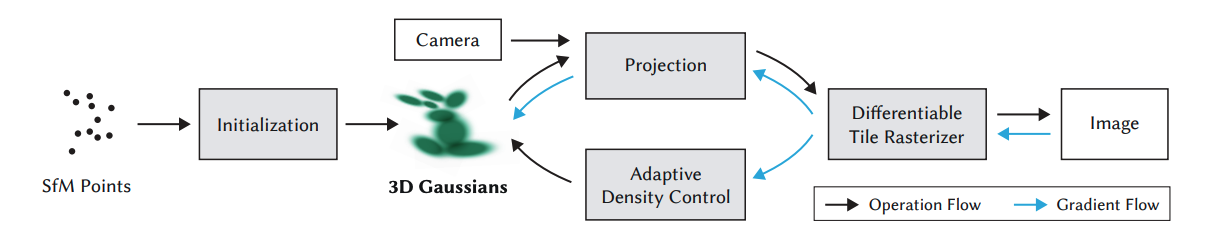
\includegraphics[width=\textwidth]{figures/fig7_3dgs_pipeline.png}
\caption{Pipeline overview of 3DGS \cite{ref4}}
\label{fig:7}
\end{figure}

\textbf{SfM Initialization}: The 3DGS process begins with a sparse reconstruction obtained via Structure-from-Motion (often using COLMAP). This provides an initial set of 3-D point estimates $\{P_i\}$ and camera poses $\{T_j\}$ for the images. Each point $P_i$ is a 3-D position corresponding to a real-scene feature and has an associated color (from image observations). These points are crucial for initialization -- rather than starting from scratch, 3DGS ``bootstraps'' its model from this point cloud, ensuring that Gaussians begin near the correct surfaces and cover the scene sparsely. Formally, we initialize one Gaussian for each point $P_i$. The Gaussian's mean $\mu_i$ is set to the 3-D coordinates of $P_i$. Its covariance $\Sigma_i$ can start as a small kernel or be oriented based on local geometry if normal estimates are available. The color $c_i$ is initialized from the point's observed color, and opacity $\alpha_i$ can start at a default value (since SfM provides no direct opacity).

\textbf{Gaussian Optimization}: Once initialized, the Gaussians are iteratively optimized to minimize the reconstruction error against the input images. In each training iteration, a differentiable rasterization of the Gaussian splats is compared to a ground-truth image, and the Gaussian parameters are updated via gradient descent. The parameters being optimized include each Gaussian's position $\mu_i$ (to fine-tune depth and alignment), covariance $\Sigma_i$ (allowing it to stretch or shrink to better cover the local surface or volume), color $c_i$, and opacity $\alpha_i$. The loss is typically a photometric error (e.g., mean-squared error or perceptual loss) between the rendered image and the input image for each pixel. Crucially, 3DGS employs adaptive density control: the set of Gaussians is not fixed. If a region is under-fit (high loss), the algorithm can split or clone Gaussians to increase local detail. For example, a Gaussian that is too large and blurry might be split into smaller Gaussians, or if it is small but insufficient in number, it can be cloned to cover similar nearby areas. Conversely, Gaussians that become very transparent (low $\alpha$, contributing little) are pruned to keep the model efficient. This dynamic adjustment yields a dense set of primitives capable of representing fine scene details. By the end of optimization, millions of Gaussians may be present, collectively encoding the scene's radiance field.

\textbf{Differentiable Rendering}: The rendering of Gaussians is accomplished via splatting: projecting each 3-D Gaussian onto the 2-D image plane as a splat (an ellipse determined by projecting the Gaussian's covariance). A simplified formulation for the contribution of a single Gaussian $i$ to a pixel:
\begin{equation*}
w_i = e^{-\frac{1}{2}(\mathbf{x}-\mathbf{x}_i)^{\top}\left(\Sigma_i^{\mathrm{proj}}\right)^{-1}(\mathbf{x}-\mathbf{x}_i)}
\end{equation*}

where $\mathbf{x}$ is the pixel coordinate and $\mathbf{x}_i$ is the projected center of the Gaussian (with $\Sigma_i^{\mathrm{proj}}$ being the 2-D covariance of the Gaussian's footprint on the image). This weight $w_i$ determines how much Gaussian $i$ influences that pixel's color. During rendering, all Gaussians are considered in approximate back-to-front order: nearer Gaussians occlude farther ones. The pixel color is obtained by alpha compositing the contributions of visible Gaussians.

This is derived from the 3D Gaussian formula (where the covariance $\Sigma$ here is 3D) in \cite{ref4}:
\begin{equation*}
G(x) = e^{-\frac{1}{2}(x)^{T}\Sigma^{-1}(x)}
\end{equation*}

The rendering is made differentiable by ensuring the splatting operation and compositing are smooth with respect to Gaussian parameters. In practice, visibility-aware rasterization algorithms are used to accelerate this process -- they downweight Gaussians that are not visible to a camera and efficiently accumulate contributions from those that are. So that, by adjusting the Gaussians' parameters, the rendered image can be made to match the input photo; gradients from this comparison propagate to move and color the Gaussians appropriately.

\section{Code}

\subsection{exposure\_gaussians.py}

\lstinputlisting{code/exposure_gaussians.py}

\subsection{exposure\_factors.py}

\lstinputlisting{code/exposure_factors.py}

\subsection{exposure\_render.py}

\lstinputlisting{code/exposure_render.py}

\subsection{exposure\_adjustment.py}

\lstinputlisting{code/exposure_adjustment.py}

\subsection{Exposure\_losses.py}

\lstinputlisting{code/exposure_losses.py}

\subsection{neighbors.py}

\lstinputlisting{code/neighbors.py}

\subsection{exposure\_\_init\_\_call.py}

\lstinputlisting{code/exposure_init_call.py}

\subsection{trainv1.py}

The stand-alone exposure model used by trainv1.py:

\lstinputlisting{code/v1_exposure_model.py}

The training script:

\lstinputlisting{code/trainv1.py}

\subsection{trainv2.py}

\lstinputlisting{code/trainv2.py}

\subsection{render\_exposure.py}

\lstinputlisting{code/render_exposure.py}

\clearpage
\section{SSIM and PSNR Log}

\noindent (a) Results for 3DGS 2023

\noindent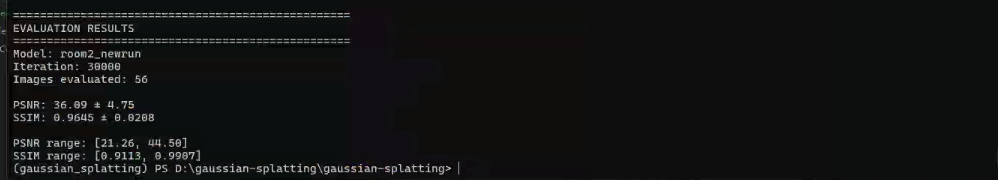
\includegraphics[width=1.0\textwidth]{figures/log_a_3dgs2023.png}

\noindent (b) Results for 3DGS 2024

\noindent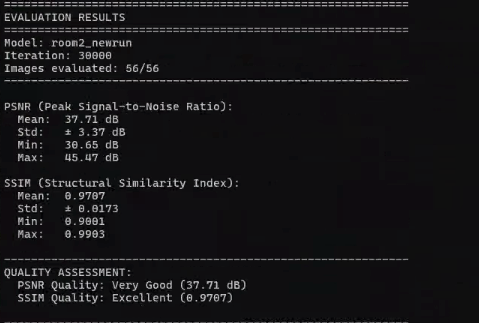
\includegraphics[width=0.8\textwidth]{figures/log_b_3dgs2024.png}

\noindent (c) Results for ours (v1)

\noindent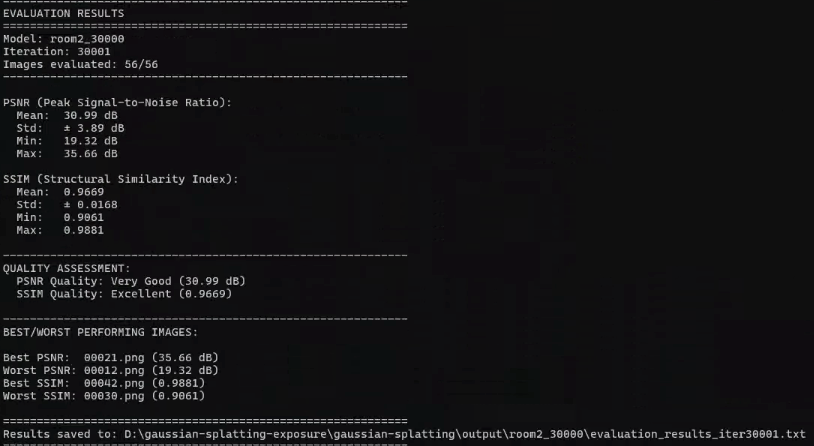
\includegraphics[width=0.95\textwidth]{figures/log_c_ours_v1.png}

\noindent (d) Results for ours (v2)

\noindent\pending{Evaluation log of trainv2.py.}

\end{document}
